Implementeringen af tilslutningsprintet er lavet ved at konstruere et veroboard print. Tilslutningsmulighederne på printet består af en indgang til 12 VDC fra PSUen, en USB-udgang der forsyner Enheden, 12 harwinstik til de forskellige sensorer og en udgang der styrer sprinklerrelæet. På figur \ref{lab:Tilslutningsprint} kan det færdige resultat ses. 

\begin{figure}[htb]
\centering
{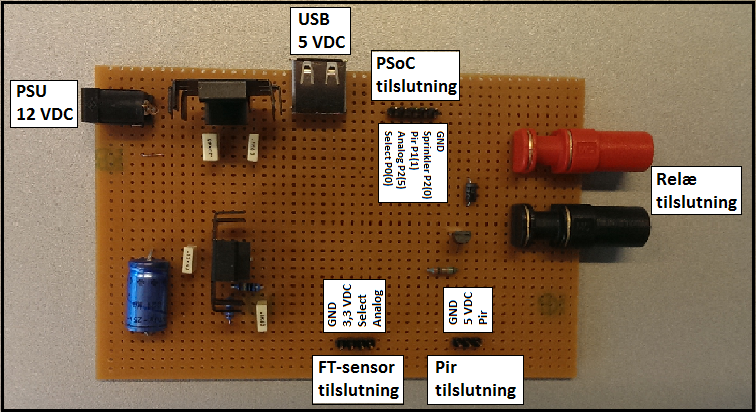
\includegraphics[width=0.70\textwidth]{filer/pics/Tilslutningsprint}}
\caption{Tilslutningsprint til forbindelse af sensorer og PSoC4}
\label{lab:Tilslutningsprint}
\end{figure}


